\documentclass{scrartcl}
\usepackage{etex}
\usepackage[ngerman]{babel}
\usepackage[utf8]{inputenc}
\usepackage[T1]{fontenc}
\usepackage{amsmath, amssymb}
\usepackage{graphicx}

\usepackage{pgfplots}
\pgfplotsset{compat=1.11}
\usepgfplotslibrary{external}
\usepackage{pgfplotstable}

\usepackage{booktabs}
\usepackage{multirow}
\usepackage{longtable}
\usepackage{ulsy}
%\usepackage{pst-all}
\usepackage{picture}
\usepackage[automark]{scrpage2}
\usepackage{caption}
\pagestyle{scrheadings}
\ihead[]{Friedrich Hübner 2897111}
\ohead[]{Fiona Paulus 2909625} 

\author{Friedrich Hübner 2897111\\
Fiona Paulus 2909625}
\title{Computerphysik\\Hausarbeit 1\\Aufgabe 2}

\begin{document}
\maketitle
\newpage

\section{Simulation}
Die Simulation der Photonen wird in aufgabe2.cpp implementiert.
\subsection{Simulation eines Photons}
Es wird, wie in der Aufgabenstellung angegeben, vorgegangen. Man startet mit einem Photon bei $\vec{p} = 0$ und berechnet in jedem Schritt einen zufälligen Richtungsvektor (nach dem in der Vorlesung angegebenen Algorithmus) und multipliziert den mit der freien Weglänge an dem Punkt. Um diesen Vektor wird das Photon nun verschoben. Die Gesamtstrecke wird gespeichert und am Ende mithilfe der Lichtgeschwindigkeit in die Zeit umgerechnet, die das Photon gebraucht hat.\\
Mithilfe von Debugausgaben konnte festgestellt werden, dass bei $R_{rad} = 500000km$ das Photon für 1m Abstand zum Kern $10\mu s$ (Computer 15s). Um die Zeit bis zum verlassen der Strahlungszone abzuschätzen, nehme ich jetzt eine lineare Extrapolation an: $t_\gamma = \frac{500000km}{1m} \cdot 10\mu s \approx 1.4 h$ bzw. $t_{CPU} = \frac{500000km}{1m} \cdot 15s \approx 240y$. Diese Zeit ist definitiv zu lang, um eine sinnvolle Simulation durchzuführen.  

\subsection{Änderung des Sonnenradius}
Wie in der Aufgabenstellung angegeben, wird jetzt der Sonnenradius auf einen kleineren Wert gesetzt. Um 1000 Photonen zu simulieren sind Sonnenradien im Bereich $R_{rad} = 0.01m..0.1m$ sinnvoll. Deswegen wurden für 10 verschiedene Werte in diesem Bereich mit jeweils 1000 Photonen die mittlere Entweichzeit bestimmt. Der Abstand zweier Sonnenradien ist durch einen konstanten Faktor gegeben, damit die Abstände Äquidistant im logarithmischen Diagramm sind. Die Ausgabe erfolgt in die Datei 'output.txt', wobei jeweils in der erste Spalte die Radien (in m) und in der zweiten Zeile die mittlere Zeit (in s) stehen. 

\section{Durchführung der Regression}
In der Datei aufgabe2\_fit.cpp wurde der Fit einer Potenzfunktion an die Daten implementiert. Dieses Programm ist vollkommen unabhängig von der Simulation. Der Potenzfunktionenfit $y = c\cdot x^d$ wird berechnet, in dem zuerst alle Daten logarithmiert werden und dann ein linearer Fit (nach Vorlesung) durchgeführt wird: $ln(y) = ln(c) + d \cdot ln(x)$. Das Programm gibt dann eine Funktion aus (In diesem Fall $1.04285\cdot 10^{-5}\cdot x^{1.99283}$).\\

\section{Plot}
Diese Funktion wird zusammen mit den Datenpunkten in ein logarithmisches Diagramm gezeichnet (Gnuplot: plot.plt). Dabei ergibt sich folgendes Bild:\\

\begin{center}
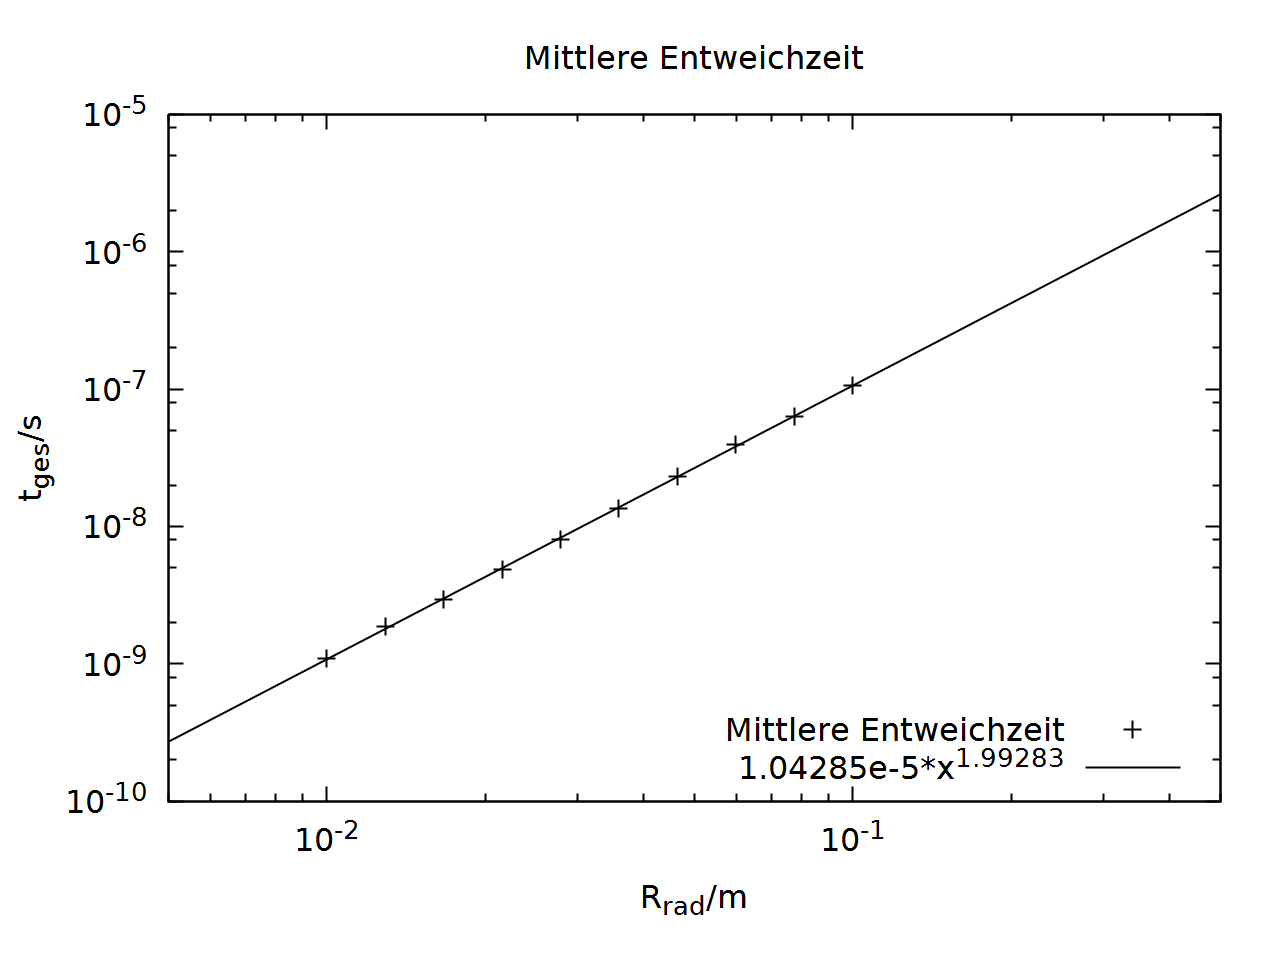
\includegraphics[scale=0.3]{plot.png}
\captionof{figure}{plot.png: Mittlere Entweichzeit über dem Radius}
\end{center}   

\section{Extrapolation}
Mithilfe einer Extrapolation kann nun die mittlere Entweichzeit bei $R_{rad} = 500000km$ bestimmt werden: $t = 1.04285e-5s\cdot (5\cdot 10^8)^{1.99283} = 2.25\cdot 10^{12} s \approx 72000y$. 

\section{Sonstige Abgegebene Dateien}
\subsection{output.txt}
Ausgabedatei der Simulation, die für das Plotten verwendet wurde.

\end{document}